\documentclass[
  journal=large,
  manuscript=propuesta,
  year=2020,
  volume=37,
]{cup-journal}

\usepackage{amsmath}
\usepackage[nopatch]{microtype}
\usepackage{booktabs}

% Correccion error: tightlist undefined sequence
\def\tightlist{}

\title{Unidad de Solidaridad y Seguros de la Cooperativa}

\author{Wong H.}
\affiliation{Ing., Organization, City, Pincode, State, Country}
\email[Wong H.]{first.author@address.edu}

\author{Joseph W.}
\affiliation{Arq., Organization, City, Pincode, State, Country}
% \alsoaffiliation{Joint first authors}

\author{}
\affiliation{}

\author{}
\affiliation{}

\addbibresource{example.bib}

\keywords{MiMutual, Gestión de usuarios, Gestión
reclamaciones} %% First letter not capped

\begin{document}

\begin{abstract}
El sistema principal de fondo Mi Mutual Central es la composición de las
funciones de negocio de la Unidad de Solidaridad de Coomeva. Las
funciones de negocio referidas, como Gestión Beneficiarios,
Certificados, Gestión Beneficiarios, aparecen dentro del componente
principal en la imagen.

Este entregable documenta los diferentes módulos y componentes que hacen
parte de la estructura de una aplicación en Angular 12 y como es su
interacción para conformar una arquitectura robusta y escalable para
aplicaciones de gran tamaño.

Las librerías Spring Boot Security y Spring Boot Oauth2 proveen
características de seguridad entre Vista (Angular 2) y Controlador.
Estas son responsables de que únicamente permita el acceso si se está
autenticado. Además, para realizar el proceso de autenticación se delega
a la aplicación SISPRO (Coomeva) que funciona como un servidor de
autenticación.
\end{abstract}

\noindent Antes SIPAS, Mi Mutual es una aplicación web compuesta por
distintos módulos de software con arreglo a todas las actividades
necesarias que soportan la operación de los productos y servicios que
ofrece la Unidad de Solidaridad y Seguros de la Cooperativa.

El despliegue es el evento que permite el inicio de las QA funcionales.

\section*{Impact Statement}
\begin{enumerate}
\def\labelenumi{\arabic{enumi}.}
\tightlist
\item
  Gestión de productos del fondo mutual y auxilio funerario que
  involucran a sus coberturas
\item
  Administración de la facturación y recaudo diario de los productos
\item
  Gestión de Reclamaciones (Indemnización): Permite realizar la gestión,
  seguimiento y pago o negación de las diferentes reclamaciones de
  acuerdo a las coberturas y los productos que se encuentren dentro del
  portafolio del Asociado.
\item
  Gestión de Beneficiarios: Permite administrar la información
  relacionada con los beneficiarios del Asociado, permitiendo ejecutar
  operaciones de consulta, inserción y modificación.
\item
  Gestión de Usuarios: Administración de la información relacionada con
  los usuarios del sistema. Este componente se comunica con el servicio
  unificado de autenticación y autorización que devuelve los permisos
  que un usuario posee sobre las opciones que proporciona el sistema.
\item
  Integración con otros sistemas para facilitar los procesos de
  vinculación, retiro, reactivación o fallecimiento de asociados.
\item
  Configuración o parametrización de factores para realizar los cálculos
  de las contribuciones de los asociados a la Cooperativa para cada uno
  de los productos adquiridos.
\end{enumerate}

\section{Insert A head here}
Antes SIPAS, Mi Mutual es una aplicación web compuesta por distintos
módulos de software con arreglo a todas las actividades necesarias que
soportan la operación de los productos y servicios que ofrece la Unidad
de Solidaridad y Seguros de la Cooperativa.

El despliegue es el evento que permite el inicio de las QA funcionales.

\CUPTWOCOL 
%%% END OF FIRST PAGE IN LARGE-LAYOUT NEEDS TO BE MARKED. This commands does nothing in medium and small layouts. %%%
Is the end of the first page. Consectetur adipiscing elit, sed do eiusmod tempor incididunt ut labore et dolore magna aliqua. Lorem ipsum dolor sit amet, consectetur adipiscing elit, sed do eiusmod tempor incididunt ut labore et dolore magna aliqua. Lorem ipsum dolor sit amet, consectetur adipiscing elit, sed do eiusmod tempor incididunt ut labore et dolore magna aliqua. Lorem ipsum dolor sit amet, consectetur adipiscing elit, sed do eiusmod tempor incididunt ut labore et dolore magna aliqua. Lorem ipsum dolor sit amet, consectetur adipiscing elit, sed do eiusmod tempor incididunt ut labore et dolore magna aliqua. 

\subsection{Insert B head here}
Subsection text here. Lorem ipsum \citep{Bayer_etal_2013} dolor sit amet, consectetur adipiscing elit, sed do eiusmod tempor incididunt ut labore \citet{Adade_etal_2007} et dolore magna aliqua. 

 Lorem ipsum dolor sit amet, consectetur adipiscing elit, sed do eiusmod tempor incididunt ut labore et dolore magna aliqua. Lorem ipsum dolor sit amet, consectetur adipiscing elit, sed do eiusmod tempor incididunt ut labore et dolore magna aliqua. Lorem ipsum dolor sit amet, consectetur adipiscing elit, sed do eiusmod tempor incididunt ut labore et dolore magna aliqua. 

\subsubsection{Insert C head here}
Subsubsection text here. Lorem ipsum dolor sit amet, consectetur adipiscing elit, sed do eiusmod tempor incididunt ut labore et dolore magna aliqua. Lorem ipsum dolor sit amet, consectetur adipiscing elit, sed do eiusmod tempor incididunt ut labore et dolore magna aliqua. Lorem ipsum dolor sit amet, consectetur adipiscing elit, sed do eiusmod tempor incididunt ut labore et dolore magna aliqua. Lorem ipsum dolor sit amet, consectetur adipiscing elit, sed do eiusmod tempor incididunt ut labore et dolore magna aliqua. Lorem ipsum dolor sit amet, consectetur adipiscing elit, sed do eiusmod tempor incididunt ut labore et dolore magna aliqua. 

Lorem ipsum dolor sit amet, consectetur adipiscing elit, sed do eiusmod tempor incididunt ut labore et dolore magna aliqua. Lorem ipsum dolor sit amet, consectetur adipiscing elit, sed do\endnote{A footnote/endnote} eiusmod tempor incididunt ut labore et dolore magna aliqua. 

\section{Equations}

Sample equations. Lorem ipsum dolor sit amet, consectetur adipiscing elit, sed do eiusmod tempor incididunt ut labore et dolore magna aliqua. Lorem ipsum dolor sit amet, consectetur\endnote{Another footnote/endnote} adipiscing elit, sed do eiusmod tempor incididunt ut labore et dolore magna aliqua. Lorem ipsum dolor sit amet, consectetur adipiscing elit, sed do eiusmod tempor incididunt ut labore et dolore magna aliqua. Lorem ipsum dolor sit amet, consectetur adipiscing elit, sed do eiusmod tempor incididunt ut labore et dolore magna aliqua. Lorem ipsum dolor sit amet, consectetur adipiscing elit, sed do eiusmod tempor incididunt ut labore et dolore magna aliqua. 


%%% Numbered equation
\begin{equation}
\begin{aligned}\label{eq:first}
\frac{\partial u(t,x)}{\partial t} = Au(t,x) \left(1-\frac{u(t,x)}{K}\right)
 -B\frac{u(t-\tau,x) w(t,x)}{1+Eu(t-\tau,x)},\\
\frac{\partial w(t,x)}{\partial t} =\delta \frac{\partial^2w(t,x)}{\partial x^2}-Cw(t,x)
+D\frac{u(t-\tau,x)w(t,x)}{1+Eu(t-\tau,x)},
\end{aligned}
\end{equation}

\begin{align}\label{eq:another}
\begin{split}
\frac{dU}{dt} &=\alpha U(t)(\gamma -U(t))-\frac{U(t-\tau)W(t)}{1+U(t-\tau)},\\
\frac{dW}{dt} &=-W(t)+\beta\frac{U(t-\tau)W(t)}{1+U(t-\tau)}.
\end{split}
\end{align}


%%%% Unnumbered equation
\begin{align*}
&\frac{\partial(F_1,F_2)}{\partial(c,\omega)}_{(c_0,\omega_0)} = \left|
\begin{array}{ll}
\frac{\partial F_1}{\partial c} &\frac{\partial F_1}{\partial \omega} \\\noalign{\vskip3pt}
\frac{\partial F_2}{\partial c}&\frac{\partial F_2}{\partial \omega}
\end{array}\right|_{(c_0,\omega_0)}\\
&\quad=-4c_0q\omega_0 -4c_0\omega_0p^2 =-4c_0\omega_0(q+p^2)>0.
\end{align*}


\section{Figures \& Tables}

The output for a single-column figure is in Figure~\ref{fig_sim}.  Lorem ipsum dolor sit amet, consectetur adipiscing elit, sed do eiusmod tempor incididunt ut labore et dolore magna aliqua. Lorem ipsum dolor sit amet, consectetur adipiscing elit, sed do eiusmod tempor incididunt ut labore et dolore magna aliqua. Lorem ipsum dolor sit amet, consectetur adipiscing elit, sed do eiusmod tempor incididunt ut labore et dolore magna aliqua.

%See Figure~\ref{fig_wide} for a double-column figure; this is always at the top of a following page.


\begin{figure}[hbt!]
\centering
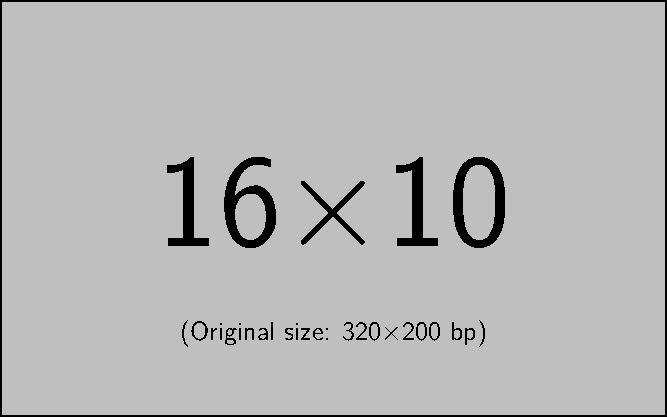
\includegraphics[width=0.75\linewidth]{example-image-16x10.pdf}
\caption{Insert figure caption here}
\label{fig_sim}
\end{figure}


\begin{figure*}
\centering
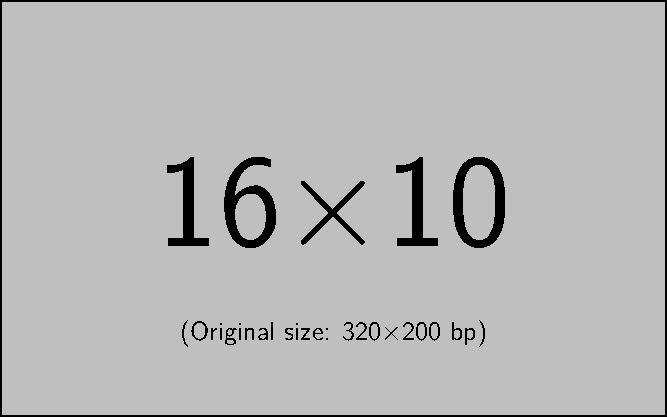
\includegraphics[width=0.8\linewidth]{example-image-16x10.pdf}
\caption{Insert figure caption here}
\label{fig_wide}
\end{figure*}


See example table in Table~\ref{table_example}.

\begin{table}[hbt!]
\begin{threeparttable}
\caption{An Example of a Table}
\label{table_example}
\begin{tabular}{llll}
\toprule
\headrow Column head 1 & Column head 2  & Column head 3 & Column head 4\\
\midrule
One\tnote{a} & Two&three three &four\\ 
\midrule
Three & Four&three three\tnote{b} &four\\
\bottomrule
\end{tabular}
\begin{tablenotes}[hang]
\item[]Table note
\item[a]First note
\item[b]Another table note
\end{tablenotes}
\end{threeparttable}
\end{table}


\section{Conclusion}
\begin{enumerate}
\def\labelenumi{\arabic{enumi}.}
\tightlist
\item
  Disponibilidad. Se requiere que el sistema esté disponible 7 X 24, el
  servicio prestado al cliente no se limita a horarios de oficina pues
  las compras pueden darse en cualquier momento
\item
  Escalabilidad. Se requiere que el sistema pueda llegar a atender hasta
  1.000 clientes, para esto se requiere que el sistema se pueda extender
  horizontalmente de tal manera que pueda tener instalado en varios
  servidores para atender esta cantidad de usuarios. Todas las
  aplicaciones desarrolladas podrán ser escaladas horizontalmente para
  atender la demanda relacionada con el crecimiento de la empresa.
\item
  Reutilización. Se requiere que el sistema permita reutilizar sus
  componentes para prestar el mismo servicio a otras aplicaciones de la
  compañía. Para esto se va a desarrollar la aplicación utilizando
  servicios, separados y con asignación de responsabilidades, propias,
  de tal manera de que, si se requiere exponer servicios web sobre estas
  funcionalidades, no requiere cambios en la aplicación.
\item
  Autenticación. Autenticación es el proceso para determinar que alguien
  o un sistema es quien dice ser. Uso de estándar Oauth2 y JSON Web
  Token -- JWT, para gestión de autenticación de servicios de la
  aplicación.
\item
  Autorización. Autorización se refiere a la validación que realiza un
  sistema para determinar si un usuario puede usar cierta funcionalidad.
  Uso de API de seguridad de Spring (spring-security) + Oauth2
\item
  Interoperabilidad -- Movilidad. Interoperabilidad se refiere a la
  habilidad de un sistema de interactuar y comunicarse con sistemas
  heterogéneos a través de interfaces completamente definidas. Uso de
  estándar de web services REST + JSON.
\item
  Facilidad de Uso. Se refiere a la facilidad con que las personas
  pueden utilizar el sistema porque facilitan la lectura de los textos,
  descargan rápidamente la información y presentan funciones y menús
  sencillos, por lo que el usuario encuentra satisfechas sus consultas y
  cómodo su uso.
\item
  Verificación (QA). Es la capacidad del producto software que hace
  posible que el software modificado sea probado.
\end{enumerate}


\begin{acknowledgement}
Agradecimientos.
\end{acknowledgement}

\paragraph{Funding Statement}

This research was supported by grants from the <funder-name> <doi> (<award ID>); <funder-name> <doi> (<award ID>).

\paragraph{Competing Interests}

A statement about any financial, professional, contractual or personal relationships or situations that could be perceived to impact the presentation of the work --- or `None' if none exist.

\paragraph{Data Availability Statement}

A statement about how to access data, code and other materials allowing users to understand, verify and replicate findings --- e.g. Replication data and code can be found in Harvard Dataverse: \verb+\url{https://doi.org/link}+.



%\endnote in some journals will behave like \footnote; and \printendnotes will not output anything. 
\printendnotes

% \printbibliography

\appendix

\section{Example Appendix Section}

Simuladores: Funcionalidades que permiten generar las simulaciones de
los diferentes planes o modificaciones (incrementos y disminuciones) a
los productos del Asociado.

\end{document}
